\section{CTFEF}

\begin{frame}
    \frametitle{CTFEF compiler architecture}
    \begin{figure}
        
        \begin{center}
            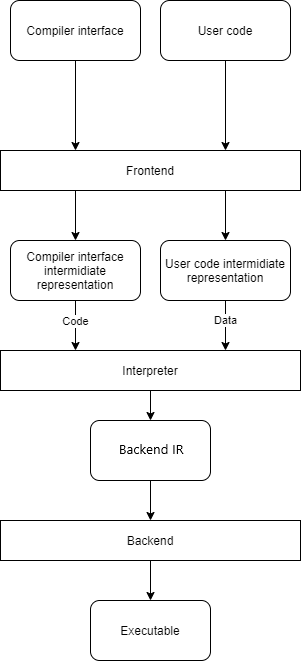
\includegraphics[height=6cm]{pictures/compiler-structure.png}
        \end{center}
    \end{figure}

\end{frame}


\begin{frame}
    \frametitle{Frontend}

    \begin{itemize}
        \item Translates source code into Intermidiate Representation\begin{itemize}
            \item Parse
            \item Validate syntax
            \item Inline operators with special syntax (ex: \lstinline|typeof|)
        \end{itemize}
        \item Processes user code and Compiler Interface\begin{itemize}
            \item Compiler interface translates user code into backend Intermidiate Representation
        \end{itemize}
        \item May perform additional processing\begin{itemize}
            \item In C-=-1 it invokes the interpreter to execute metaprogramming code
        \end{itemize}
    \end{itemize}

\end{frame}

\begin{frame}
    \frametitle{Intermidiate Representation}

    \begin{itemize}
        \item Complete representation of the user program
        \item Simplified form of the compiled language\begin{itemize}
            \item Resolved function overloads
            \item Advanced constructs lowered to basic ones (foreach loops transformed into while)
        \end{itemize}
        \item Stored using Interpreter data structures in compiler memory\begin{itemize}
            \item 
        \end{itemize}
    \end{itemize}

\end{frame}

\begin{frame}
    \frametitle{Interpreter}

    \begin{itemize}
        \item Operates on Intermidiate Representation
    \end{itemize}

\end{frame}
